\chapter{Introducción}
\label{cap:capitulo1}
\setcounter{page}{1}

Desde sus inicios, la robótica ha proporcionado un sinfín de posibilidades y alternativas ante problemas que anteriormente carecían de las soluciones adecuadas, pero, ¿qué es realmente la robótica?\\

Se podría definir robótica como el proceso mediante el cual una máquina intercambia energía e información con su entorno, con el propósito de alcanzar una serie de objetivos específicos. Este campo tecnológico en expansión es el resultado de décadas de colaboración contínua entre biólogos, informáticos e ingenieros \cite{Koditschek21}.

Dada esta multidisciplina, la robótica abarca una amplia gama de aplicaciones, desde la industria hasta la medicina, pasando por la exploración espacial, la domótica o la conducción autónoma, entre otras. Es un campo en constante evolución, impulsado por la búsqueda de soluciones innovadoras para mejorar la calidad de vida y permitir superar desafíos de manera más eficiente y segura.\\

La industria agrícola no es una excepción, ya que ha contemplado históricamente tareas que requieren una dedicación laboral considerable. No obstante, gracias a la robótica y a los sistemas de visión artificial, surge la oportunidad de transformar una serie de procesos, como puede ser la recolección de cultivos, a través de la detección automatizada para su posterior recolección.\\

En las siguientes secciones describiremos brevemente algunas de las aplicaciones más importantes de la robótica en la sociedad actual, así como los distintos conceptos en los cuales se basa la investigación y el desarrollo llevado a cabo.\\

\section{Robots y robótica}
\label{sec:robótica} % etiqueta para luego referenciar esta sección

Según la Federación Internacional de Robots (IFR) se define robot según el vocabulario establecido por la International Organization for Standardization (ISO), y esto es como \textit{"mecanismo accionado programado con cierto grado de autonomía para realizar tareas de locomoción, manipulación o posicionamiento"} \cite{ISO8373}.\\  

El término “robot” fue utilizado por primera vez por Karel Capek (en su obra de teatro “Rossum’s Universal Robots” publicada en 1920. Esta palabra viene del vocablo checo \textit{“robota”} que significa “trabajo”, en el sentido de la obligatoriedad, entendido como servidumbre, trabajo forzado o esclavitud \cite{Sanchez07a}.

Aunque esta definición es un punto de partida, es cierto que es posible diferir en aspectos como si un robot debe controlarse automáticamente o podría ser autónomo o si un robot debe ser reprogramable. A un nivel más amplio, cualquier máquina que pueda utilizarse para llevar a cabo acciones o tareas complejas de forma automática puede considerarse un robot \cite{Raj19}.\\

Históricamente, las civilizaciones antiguas, como la egipcia y la griega, dieron los primeros pasos en lo que se puede denominar robótica clásica, construyendo autómatas y mecanismos diseñados para imitar acciones humanas, con características mecánicas rudimentarias. 
Con el paso del tiempo, la ciencia y la ingeniería avanzaron, y los conceptos de la robótica comenzaron a tomar forma más definida hasta que, en el siglo XX, con el desarrollo de la ingeniería en sus diferentes ramas (mecánica, electrónica, informática, telecomunicaciones), Isaac Asimov (1920-1992) utilizó por primera vez el término “robótica” y postuló las tres leyes de la robótica en su libro \textit{I Robot} publicado en 1950, coincidiendo con el apogeo de la robótica moderna. Asimov consideró necesario añadir una cuarta ley, antepuesta a las demás, la número cero, que afirma que un robot no debe actuar simplemente para satisfacer intereses individuales, sino que sus acciones deben preservar el beneficio común de toda la humanidad \cite{Sanchez07b}.

\pagebreak

\begin{table} [h!]
  \begin{center}
    \begin{tabular}{p{15cm}} % Ajustar el ancho según necesidades
      \hline
      1. Un robot no debe dañar a un ser humano ni, por su pasividad, dejar que un ser humano sufra daño.\\\\
    
      2. Un robot no debe obedecer las órdenes que le son dadas por un ser humano, excepto cuando estas órdenes están en oposición con la primera Ley.\\\\
    
      3. Un robot debe proteger su propia existencia, hasta donde esta protección no esté en conflicto con la primera o segunda Ley. \\
      \hline
    \end{tabular}
  \end{center}
  \caption{Las tres leyes de la robótica según Asimov.}
  \label{cuadro:leyesrobotica_Asimov}
\end{table}

Es también en 1950, cuando Alan Mathison Turing publica \textit{“Computing Machinery and Intelligence”} y propone una prueba (test o máquina de Touring), en forma de entidad matemática abstracta, que demuestra la existencia de problemas computacionales irresolubles que ninguna máquina es capaz de solventar. Se puede afirmar que un programa de ordenador no llegará nunca a ser tan inteligente como un ser humano y que un robot no podrá suplir al ser humano de forma completa, \cite{Sanchez07b} preocupación sobre el potencial de sustitución de la mano de obra, que históricamente, ha atenuado el entusiasmo en torno a las nuevas tecnologías \cite{Mokyr15}.\\

Partiendo de todos estos avances y del interés por automatizar las tareas de producción, la robótica va adquiriendo un gran desarrollo \cite{Sanchez07b}. Es debido a este desarrollo, que atendiendo al propósito y al contexto en el que se utilicen estos robots, se fueron creando varios grupos en función de los que clasificarles. Estos tres grandes grupos en función de una serie de criterios generales fueron: robots industriales, robots de servicio y robots médicos.

\subsection{Robot Industrial}
\label{sec:robot_industrial}

Se define robot industrial como un "manipulador polivalente, reprogramable y controlado automáticamente, programable en tres o más ejes, que puede ser fijo o móvil para su uso en aplicaciones de automatización industrial" \cite{ISO8373}.\\

El inicio de la robótica industrial, puede datarse en la década de 1950, aunque algunos tipos de automatización en el entorno industrial empezaron a aparecer desde los tiempos de la Revolución Industrial. La evolución de los robots industriales puede subdividirse en cuatro categorías: las tres primeras abarcan el período comprendido entre los años cincuenta y finales de los noventa, mientras que la cuarta generación abarca desde 2000 hasta nuestros días \cite{Gasparetto19}.


La primera generación o primeros manipuladores (1950-1967) eran básicamente máquinas programables que no tenían comunicación con el entorno externo y con algoritmos de control sencillos (punto a punto). En cuanto al hardware, contaban con equipos de baja tecnología, sin servocontroladores. Sin embargo, en 1954, George Devol y Joseph Engelberger formaron la empresa Unimation, empresa que desarrollaría Unimate, considerado el primer robot industrial de la historia, fabricado en 1961 \cite{Zamalloa17}.
  
  \begin{figure}[h!]
    \begin{center}
      \subcapcentertrue
      \subfigure[Joseph Engelberger y George Devol]{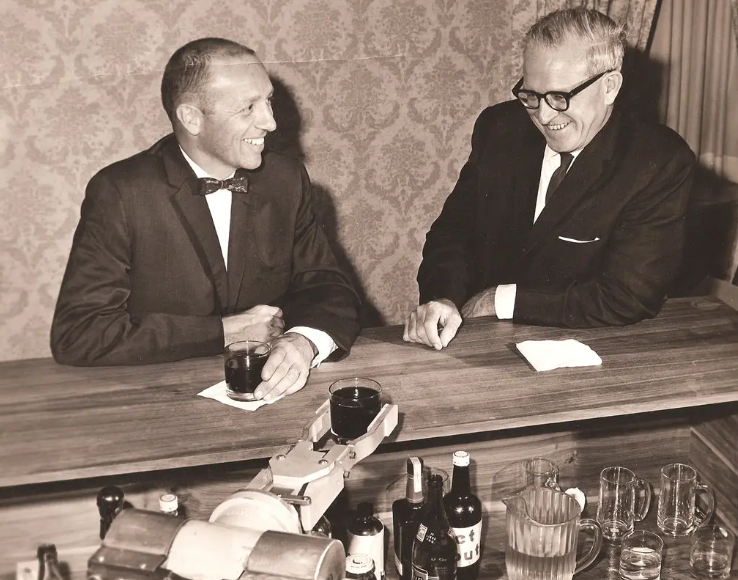
\includegraphics[width=62mm]{figs/Engelberger_Devol.png}}
      \hspace{2mm}
      \subfigure[Robot Unimate]{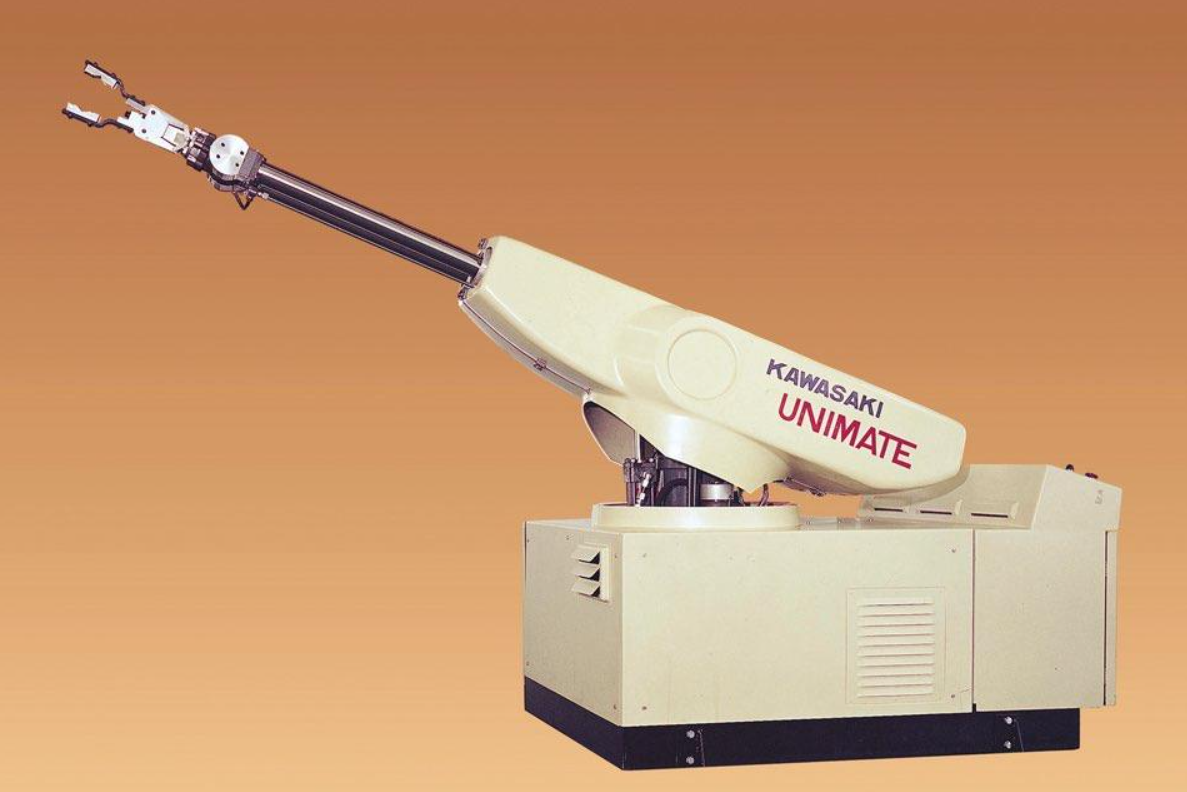
\includegraphics[width=73mm]{figs/Unimate robot.png}}
    \end{center}
    \caption{Primer robot industrial.}
    \label{fig:primer_robot_industrial}
  \end{figure}
  
Empresas como Ford y General Motors empezaron a plantearse la automatización de sus plantas productivas, por lo que, en 1962, la empresa AMF Corporation fabricó un nuevo robot llamado Versatan, un robot cilíndrico que Ford encargó para sus fábricas. Este robot, fue también el primero que se instaló en un centro productivo en Japón \cite{Gasparetto19}. \\

La segunda generación o robots sensorizados (1968-1977) eran máquinas programables básicas con posibilidades limitadas de comportamiento autoadaptativo y capacidades elementales para reconocer el entorno externo, poseían sistemas sensoriales avanzados y eran robots de gran volumen que se utilizaban principalmente en automoción \cite{Zamalloa17}. \\

En 1968, en el Stanford Artificial Intelligence Laboratory (SAIL) se confecciona el WAVE, el primer lenguaje de programación para robots. En 1969, Unimation concendió a Kawasaki Heavy Industries Ltd. la licencia para producir robots para el mercado japonés y asiático, conduciendo al desarrollo del Kawasaki-Unimate 2000, el primer robot industrial construido en Japón. Es también en este año cuando Víctor Scheinman, un estudiante de ingeniería mecánica de la Universidad de Standford, diseñó y construyó el primer prototipo de brazo robótico, cuya cinemática inversa podía resolverse de manera analíticamente cerrada, permitiendo una rápida ejecución de la trayectoria \cite{Gasparetto19}. 

  \begin{figure}[h!]
    \begin{center}
      \subcapcentertrue
      \subfigure[Victor Scheinman con el Standford Arm]{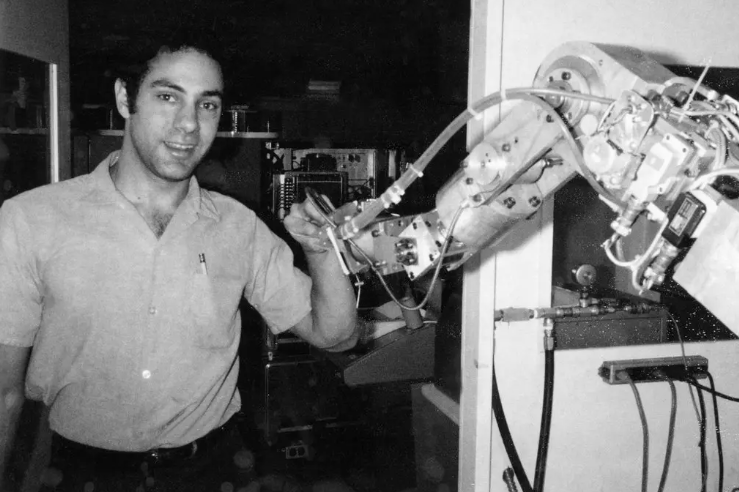
\includegraphics[width=62mm]{figs/Victor_Scheinman.png}}
      \hspace{2mm}
      \subfigure[Standford Arm]{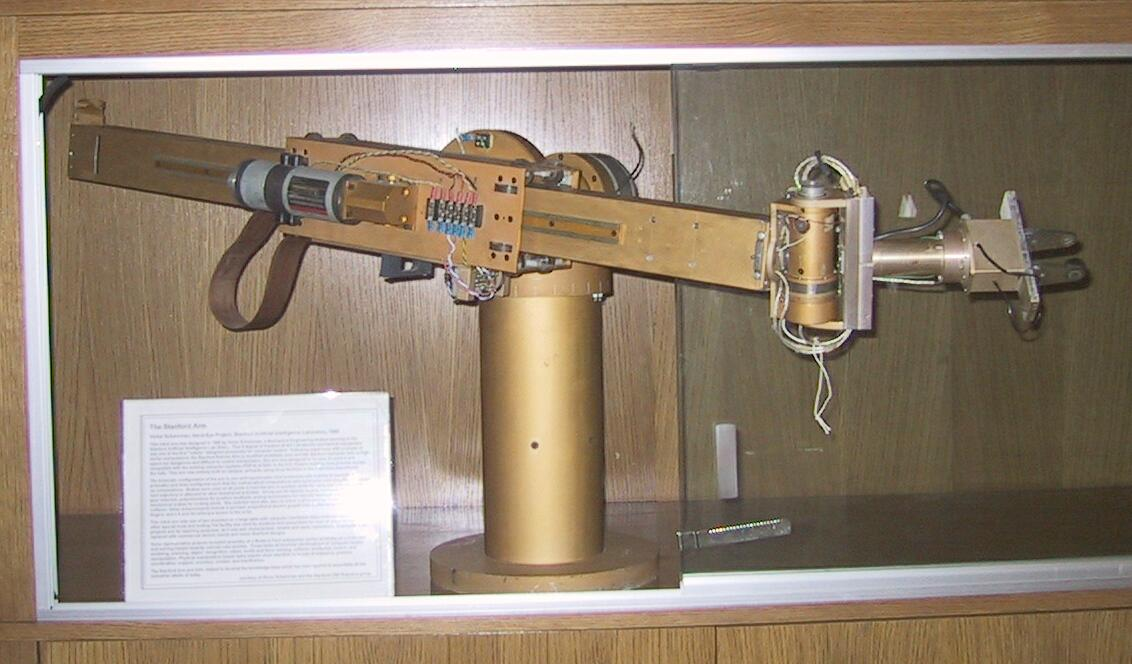
\includegraphics[width=71mm]{figs/Standford_arm.jpeg}}
    \end{center}
    \caption{Standford Arm.}
    \label{fig:standford_arm}
  \end{figure}
 
El ingeniero de la compañía Yaskawa, T Mori, en 1969 acuña el término mecatrónica que integra el conjunto de mecanismos de control automático imprescindibles para el desarrollo de cualquier máquina inteligente \cite{Sanchez07b}.
  
  \begin{figure} [h!]
    \begin{center}
      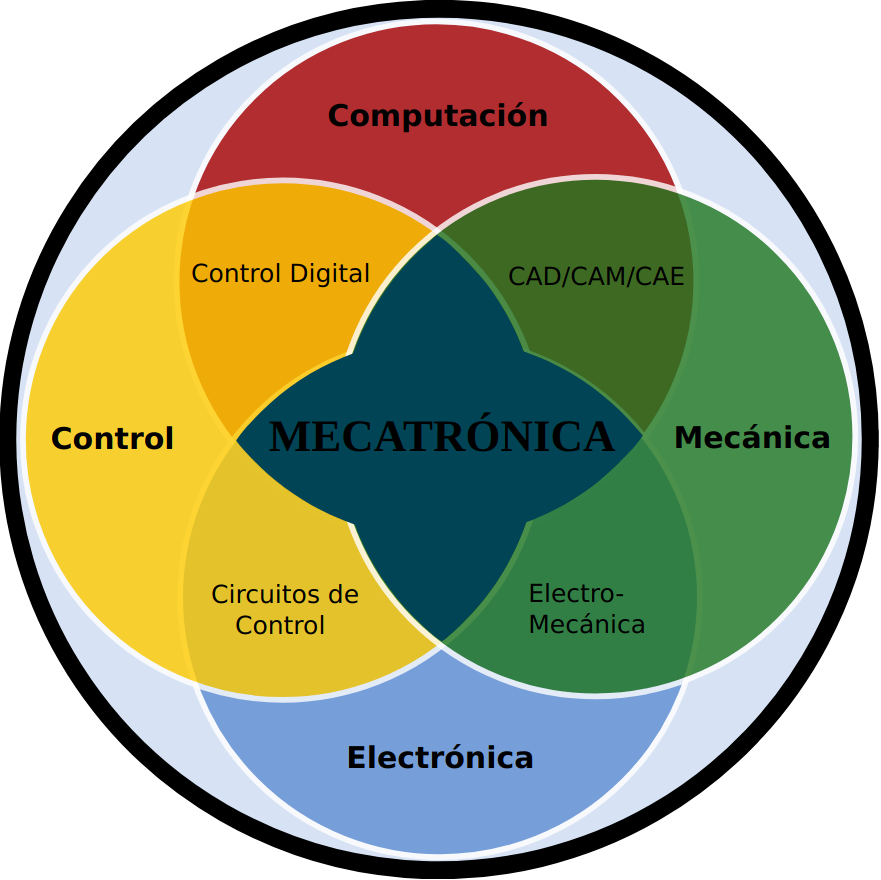
\includegraphics[width=65mm]{figs/meca.png}
    \end{center}
    \caption{Diagrama mecatrónico de construcción de máquinas inteligentes.}
    \label{fig:Mecatrónica}
  \end{figure}
  
En 1973, KUKA construyó el primer robot industrial con 6 ejes electromecánicos llamado Famulus. Un año más tarde, Cincinnati Milacron introdujo en el mercado el robot T3. Cincinnati Milacron (adquirida por ABB en 1990). El robot T3 fue el primer robot comercial controlado por un microordenador \cite{Zamalloa17}.
  
  \begin{figure} [h!]
    \begin{center}
      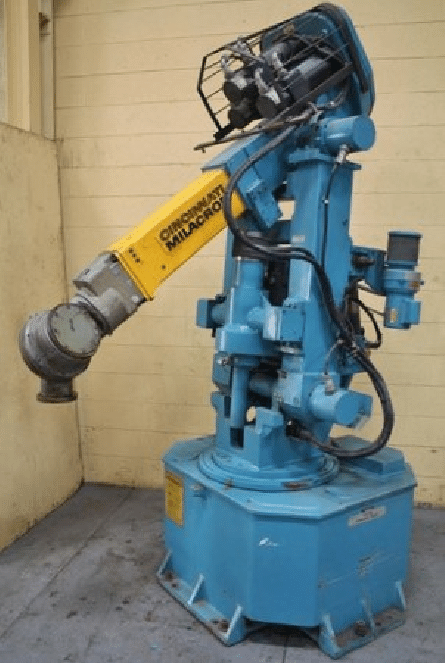
\includegraphics[width=55mm]{figs/T3_robot.png}
    \end{center}
    \caption{Robot Cincinnati Milacron T3.}
    \label{fig:T3}
  \end{figure}
  
  \pagebreak
  
La tercera generación o robots industriales (1978-1999) disponían de controladores específicos (ordenadores), siendo un punto clave en la caracterización de este generación, además del surgimiento de nuevos lenguajes de programación para el control de los robots, la posibilidad de reprogramarlos y la inclusión parcial de la visión artificial \cite{Zamalloa17}. Entre finales de los años setenta y principios de los ochenta, otros avances científicos y técnicos contribuyeron a la difusión de los robots \cite{Gasparetto19}, que junto a que las empresas de todo el mundo invirtieron miles de millones de dólares en del mundo para automatizar tareas básicas en sus cadenas de montaje, supusieron que los robots poblaran muchos sectores industriales para automatizar una amplia variedad de actividades \cite{Zamalloa17}.\\ 

Unimation diseñó y fabricó en 1978 el robot PUMA. El PUMA (acrónimo de Programmable Universal Machine for Assembly) fue considerado durante muchas décadas el arquetipo de los robots antropomórficos \cite{Gasparetto19}. En 1978, el científico japonés Hiroshi Makino, de la Universidad de Yamanashi, propuso una nueva estructura cinemática. El robot con esta estructura se denominó SCARA (acrónimo de "Selective Compliance Assembly Robot Arm"), ya que su conformidad en la dirección horizontal resultó menor que la conformidad en la dirección vertical. Por esta razón, así como por la ligereza de la cadena cinemática (que permitía un controlador más sencillo y rápido), este robot era adecuado para ser empleado en tareas como el ensamblaje de objetos pequeños \cite{Makino80}.
  
  \begin{figure} [h!]
    \begin{center}
      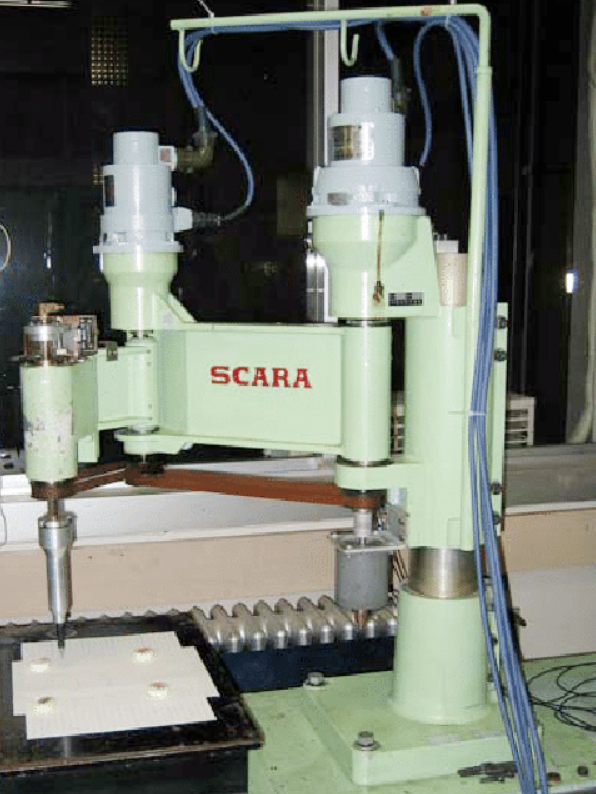
\includegraphics[width=45mm]{figs/Scara.png}
    \end{center}
    \caption{Uno de los primeros prototipos de robot SCARA.}
    \label{fig:Scara}
  \end{figure}
  
  \pagebreak
  
Más tarde, en 1981 en la Universidad Carnegie-Mellon se desarrolló un robot de impulsión directa que utiliza motores eléctricos en las articulaciones, evitando la distorsión de las transmisiones mecánicas convencionales. En 1982, IBM introduce el robot de montaje industrial RS-1 que utiliza un brazo constituido por 3 dispositivos de deslizamiento \cite{Sanchez07b}. De la idea de emplear cadenas cinemáticas paralelas en lugar de las clásicas cadenas cinemáticas en serie, junto con la de crear un robot ligero capaz de moverse a gran velocidad, surgió el arquetipo del robot Delta (que apareció en 1992), concebido por el científico suizo Reymond Clavel en la Escuela Politécnica Federal de Lausana (EPFL) \cite{Clavel91}. En comparación con los robots en serie, los robots paralelos tienen un espacio de trabajo más pequeño, pero pueden funcionar a una velocidad mucho mayor, siendo la arquitectura cinemática ideal para los robots dedicados a operaciones de pick-and-place de alta velocidad. Basado en este tipo de estructura, unos años después, en 1998, ABB desarrolló el Flex-Picker, el robot de picking más rápido del mundo \cite{Gasparetto19}.\\
  
  \begin{figure} [h!]
    \begin{center}
      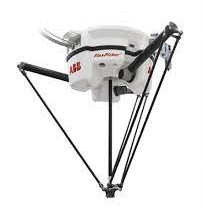
\includegraphics[width=45mm]{figs/flexpicker_ABB.jpeg}
    \end{center}
    \caption{Robot ABB IRB 360 Flexpicker.}
    \label{fig:Flexpicker_ABB}
  \end{figure}
  
A partir de los años 2000, aparece la cuarta generación o robots inteligentes (2000-Actualidad), que se caracteriza por la inclusión de capacidades informáticas avanzadas, ya que los ordenadores no sólo trabajan con datos, si no también pueden realizar razonamientos lógicos y aprender, puesto que la Inteligencia Artificial comienza a ser incluida parcial y experimentalmente en estos robots. Los sensores son más sofisticados, y envían información al controlador y la analizan mediante estrategias de control complejas para que el robot pueda basar sus acciones en información sólida y fiable. Es en esta generación cuando se introducen los robots colaborativos \cite{Zamalloa17}.\\
  
Los requisitos de velocidad y peso de un robot han dado lugar a novedosos diseños cinemáticos y de transmisión. Desde el principio, la reducción de la masa y la inercia de las estructuras robóticas ha sido un objetivo primordial en el desarrollo de la robótica. El brazo humano, con una relación peso-carga de 1:1, se consideraba la referencia definitiva \cite{Siciliano16}. Con este objetivo, se desarrollaron gracias a la colaboración entre la empresa alemana KUKA y el Instituto de Robótica y Mecatrónica del Centro Aeroespacial Alemán (DLR), tres generaciones de robots ligeros, permitiendo a investigadores e ingenieros desarrollar nuevas aplicaciones de robótica industrial y de servicios con un rendimiento sin precedentes. En el año 2004, con motivo de Automática, la mayor exposición de robots del mundo, se presentó por primera vez la combinación entre el robot ligero del DLR y la controladora KUKA, denominado RoboAssistant, donde se permitió a los visitantes mover y programar manualmente el robot, haciendo la visión de un robot que asiste a un trabajador durante los procesos de producción evidente para los visitantes \cite{Bischoff10}. \\
  
  
Es en estos procesos de producción, donde la manipulación a dos manos puede ser crítica para tareas de ensamblaje complejas, manipulación simultánea
y procesamiento de piezas de trabajo o para la manipulación de objetos de gran tamaño, por lo que en 2005, MOTOMAN presenta el primer robot comercial para la manipulación sincronizada a dos manos \cite{Siciliano16}.\\

  \begin{figure} [h!]
    \begin{center}
      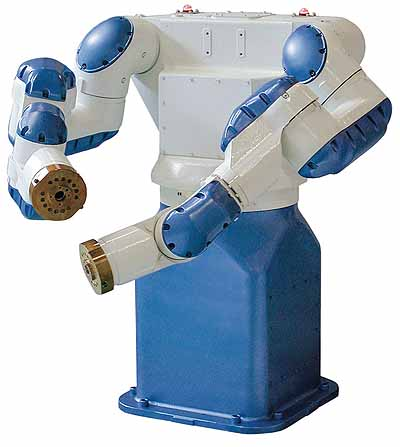
\includegraphics[width=55mm]{figs/MOTOMAN.jpg}
    \end{center}
    \caption{Robot Motoman DA-20.}
    \label{fig:MOTOMAN}
  \end{figure}
  
  \pagebreak
  
Sin embargo, fue en el año 2006 cuando, tras haber estado trabajando en la búsqueda de vías para el desarrollo en serie del robot LWR3 del DLR, y tras una intensa cooperación entre KUKA y el DLR para transmitir a los desarrolladores de KUKA los conocimientos necesarios para para el desarrollo de brazos ligeros, componentes y electrónica integrada, cuando se toma la decisión de producir una primera pequeña serie del robot ligero del KUKA LWR3 \cite{Bischoff10}.
  
  \begin{figure}[h!]
    \begin{center}
      \subcapcentertrue
      \subfigure[RoboAssistant en Automatica 2004]{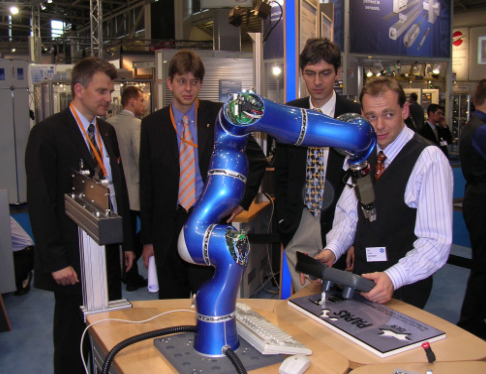
\includegraphics[width=65mm]{figs/RoboAssistant.png}}
      \hspace{2mm}
      \subfigure[Robot KUKA LWR3 con controladora (2006)]{\includegraphics[width=55mm]{figs/Kuka_lightweightrobot_2006.png}}
    \end{center}
    \caption{LWR3}
    \label{fig:Lightweight Robot (LWR)}
  \end{figure}
  
A principios de 2007, dos estudiantes de doctorado de la Universidad de Standford, Keenan Wyrobek y Eric Bergerlas, pusieron las primeras piezas de lo que eventualmente se convertiría en el Robot Operating System (ROS). Uno de los preceptos principales que se tuvo en cuenta para la creación de este Sistema Operativo para Robots fue el de crear un sistema que permitiese al máximo posible la reutilización de código, dando soporte a distintos tipos de robots y de aplicaciones. Esto resultó en la incorporación de ROS en una sorprendentemente amplia variedad de robots, extendiéndose incluso a dominios más allá de la comunidad académica de investigación a la que se dirigió inicialmente. Los años siguientes superaron todas las expectativas debido a que los avances en el ámbito de la robótica se compartieron de manera reproducible en ROS, y la Open Source Robotics Foundation (OSRF), Fundación de Robótica de Código Abierto en inglés, se convirtió en el administrador principal de ROS en 2014. Con el objetivo de atender de manera más efectiva las demandas de una comunidad ROS más extensa y abordar sus nuevos escenarios de aplicación, la OSRF se dedicó a desarrollar ROS2 como un conjunto de paquetes paralelos que pudieran ser instalados junto a ROS1 (la versión original de ROS que nació en el año 2010) y ser compatibles entre sí. Además, la popularidad de ROS ha seguido creciendo en la industria con el apoyo de proyectos como ROS-Industrial (ROS-I), una iniciativa de código abierto que extiende las capacidades avanzadas de ROS a hardware y aplicaciones industriales relevantes. \cite{Suarez22}.\\
  
  \begin{figure}[h!]
    \begin{center}
      \subcapcentertrue
      \subfigure[Robot PR1]{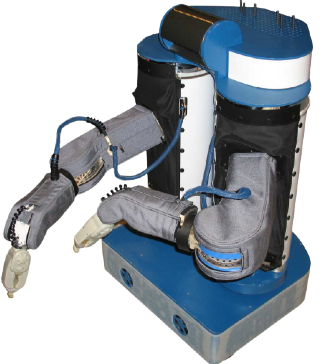
\includegraphics[width=52mm]{figs/PR1.png}}
      \hspace{2mm}
      \subfigure[Robot PR2]{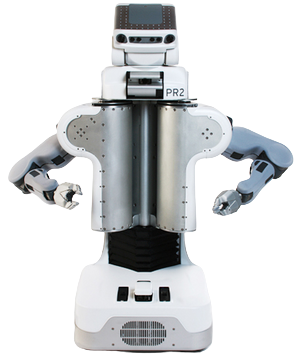
\includegraphics[width=50mm]{figs/PR2.png}}
    \end{center}
    \caption{Robots utilizados para el desarrollo de ROS.}
    \label{fig:PR_ROS}
  \end{figure}
  
  
  \begin{figure} [h!]
    \begin{center}
      
\includegraphics[width=55mm]{figs/ROS_logo.png}
    \end{center}
    \caption{Logo de ROS.}
    \label{fig:ROS}
  \end{figure}
  
  \pagebreak
  
En el año 2008 se entrega el primer robot colaborativo o cobot, el UR5 de Universal Robots, considerado como uno de los logros tecnológicos más significativos de la década en la comunidad robótica. El brazo robótico es pionero en la programación 3D fácil de usar pero sofisticada, con una interfaz de usuario intuitiva que permite a cualquier persona configurarlo y utilizarlo de forma rápida. Esta empresa, fundada en el año 2005 por Esteben Østergaard, Kasper Støy y Kristian Kassow tras conocerse en la Universidad de Dinamarca, surgió con el objetivo de hacer que la robótica sea accesible para las pequeñas y medianas empresas \cite{UR}.\\
  
Esben H. Østergaard, Director de Tecnología y cofundador de Universal Robots, tomó el trabajo original de Peskhin y Colgate, dos investigadores de la empresa automovilística Ford de los años 90, que decidieron crear un nuevo robot industrial, más pequeño y ágil que los tradicionales, que saliera de su jaula para colaborar estrechamente con el ser humano en las tareas de calidad y personalización de los productos, sin embargo, no fueron capaces, puesto que el problea estaba en la relación entre seguridad y rendimiento, ya que el aumento de la primera reducía el de la segunda. Østergaard consiguió diseñar un sistema de seguridad y control para el cobot que lo bloquea en caso de colisión con el operario. Como recuerda el propio Østergaard, la seguridad era la clave con la que la robótica colaborativa podía entrar en el escenario industrial. Así se creó un robot capaz de operar en espacios confinados, en estrecho contacto con humanos, y sin instalar costosas barreras de seguridad \cite{Cusano22}.
  
  \begin{figure} [h!]
    \begin{center}
      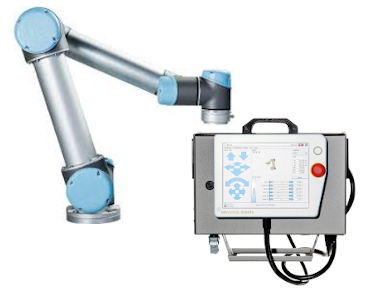
\includegraphics[width=72mm]{figs/UR5_controller.png}
    \end{center}
    \caption{UR5 con su controladora.}
    \label{fig:UR5}
  \end{figure}
  
Más tarde, en 2018, Universal Robots presenta los robots colaborativos e-Series, que incluían avances tecnológicos que permitían un desarrollo más rápido para una mayor variedad de aplicaciones, ofrecía una programación más sencilla y seguía las normas de seguridad ISO más actuales y recientes \cite{UR}.
 
  \begin{figure}[h!]
    \begin{center}
      \subcapcentertrue
      \subfigure[UR presenta los  nuevos e-Series en Automatica 2018]{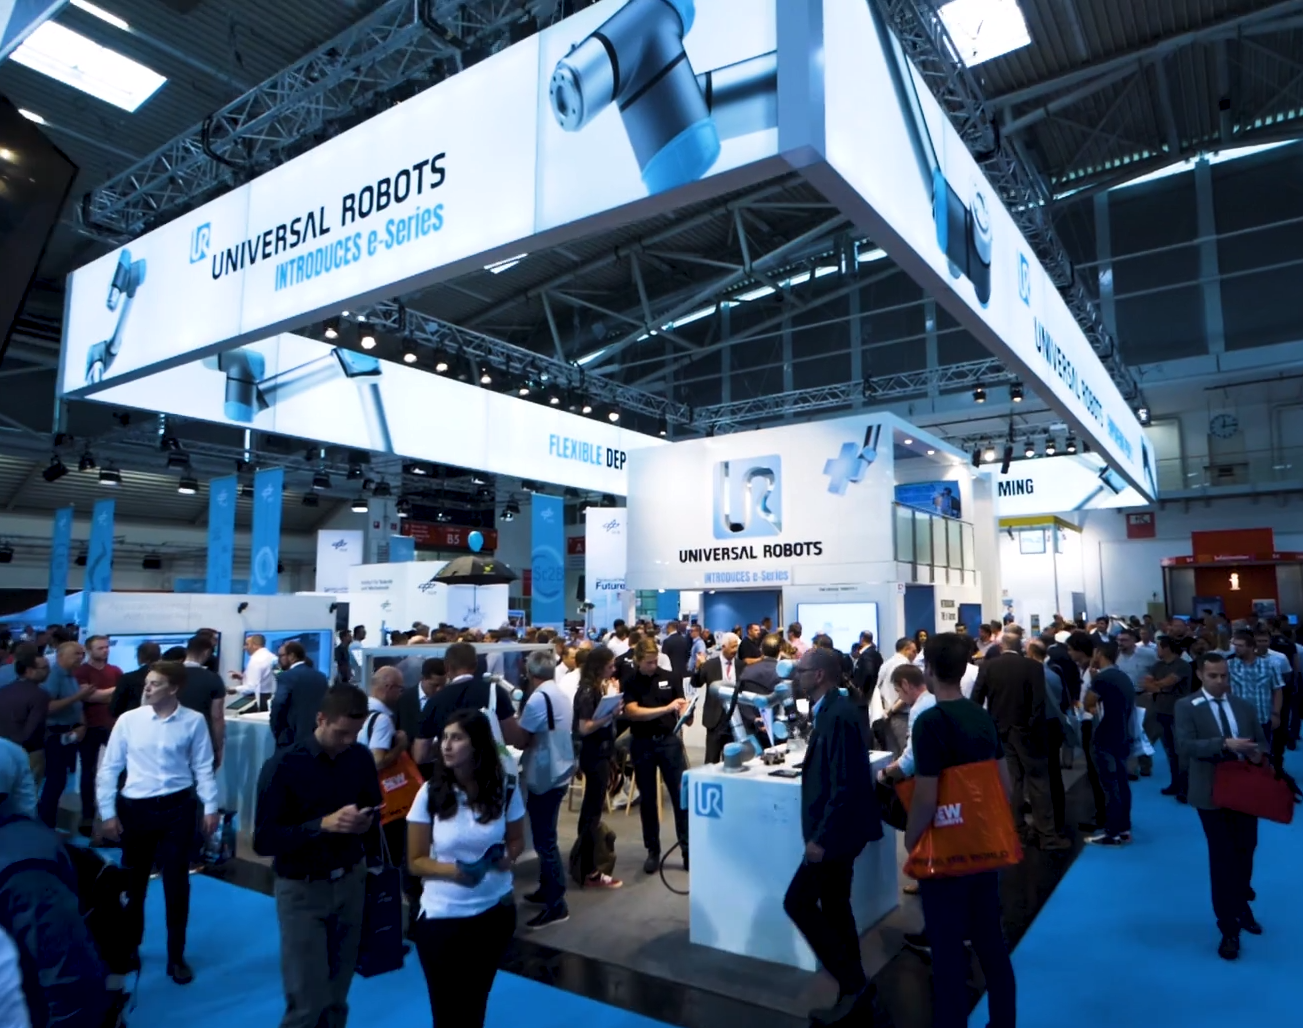
\includegraphics[width=72mm]{figs/UR Automatica 2018.png}}
      \hspace{2mm}
      \subfigure[UR e-Series]{\includegraphics[width=72mm]{figs/UR e-series.jpg}}
    \end{center}
    \caption{Universal Robots e-Series}
    \label{fig:UR_e-Series}
  \end{figure}
  
  \pagebreak	
  
Esta cuarta generación de robótica industrial ha establecido un sólido punto de partida para una continua revolución en el campo de la automatización. 
Es esencial destacar que varios de los modelos de robots mencionados previamente han seguido evolucionando y mejorando con el tiempo, siendo fruto de estas mejoras, la comercialización de nuevos modelos y series. 
Debido a que la tecnología se encuentra en constante desarrollo y a la colaboración cada vez más estrecha entre humanos y robots, el futuro de la robótica industrial promete seguir transformando radicalmente nuestros métodos de trabajo y producción, abriendo así nuevas oportunidades y desafiando constantemente los límites de lo que podemos lograr en la automatización industrial, así como en los otros dos grandes grupos de la robótica, com la robótica de servicio y la robótica médica.
   

\subsection{Robot de Servicio}
\label{sec:robot_servicio}

Se define robot de servicio como un robot que realiza tareas útiles para las personas o los equipos, incluyendo en esta la manipulación o el servicio de artículos, el transporte, el apoyo físico, la orientación o información, el aseo personal, la cocina y la manipulación de alimentos y la limpieza en el ámbito personal, y la inspección, vigilancia, manipulación de objetos, transporte de personas, orientación o información, cocina y manipulación de alimentos y limpieza en el ámbito profesional \cite{ISO8373}.\\

Su historia se remonta a la década de 1960, cuando surgieron los primeros intentos de crear robots para ayudar en tareas domésticas y de atención al cliente. Uno de los precursores de estos robots de servicio en 1968 fue el robot Shakey, desarrollado por el Laboratorio de Investigación de Inteligencia Artificial de Stanford o Stanford Research Institute (SRI). Shakey, provisto e múltiples sensores y medios para desplazarse por el suelo, además de control remoto por radio \cite{Sanchez07b} podía realizar tareas de planificación, búsqueda de rutas y reordenación de objetos sencillos, siendo el primer robot móvil con capacidad para percibir y razonar sobre su entorno \cite{sri}. 

  \begin{figure} [h!]
    \begin{center}
      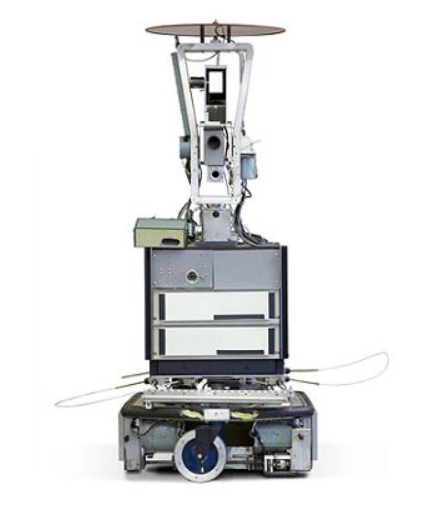
\includegraphics[width=6cm]{figs/Shakey.png}
    \end{center}
    \caption{Robot Shakey.}
    \label{fig:shakey}
  \end{figure}
   
Sin embargo, fue a mediados de los años 80 cuando en los laboratorios y centros de investigación dedicados a la robótica se trató de revitalizar la importancia de los robots en nuestra sociedad, planteando las ventajas que el uso del robot podía traer en tareas en las que el ser humano asumía riesgos o en las que las capacidades de aquel estaban limitadas por factores como la fuerza o la precisión necesaria. Fue precisamente al entenderse que estas nuevas aplicaciones de la robótica no tenían un uso industrial con el objetivo de fabricar bienes, sino que se trataba de un empleo para desarrollar tareas para las personas, cuando se catalogaron como aplicaciones en el sector servicios \cite{Barrientos02}.\\

En la práctica, las actuales y potenciales aplicaciones no industriales de los robots son tan variadas y diferentes que se dificulta su catalogación \cite{Barrientos02}, sin embargo, existen ciertas características especiales en estos robots de servicio que los hacen diferentes de los robots industriales \cite{Aracil08}, y los caracterizan para llevar a cabo estas tareas para las personas, siendo las principales características estos tres atributos de diseño: representación, antropomorfismo y orientación a la tarea, es decir, los robots de servicio pueden tener una representación física (por ejemplo, Pepper) o tener una representación únicamente virtual (por ejemplo, Alexa, ya que el software de IA virtual que funciona de forma autónoma y aprende con el tiempo también puede clasificarse como robot de servicio), diseñarse como humanoides (es decir, antropomorfos) simulando una apariencia humana o como no humanoides (por ejemplo, el robot de limpieza Roomba), y pueden realizar tareas cognitivo-analíticas gracias a la potencia informática subyacente o tareas emocionales-sociales (por ejemplo, robots de recepción) \cite{Wirtz18}.\\

 \begin{figure}[h!]
    \begin{center}
      \subcapcentertrue
      \subfigure[Alexa]{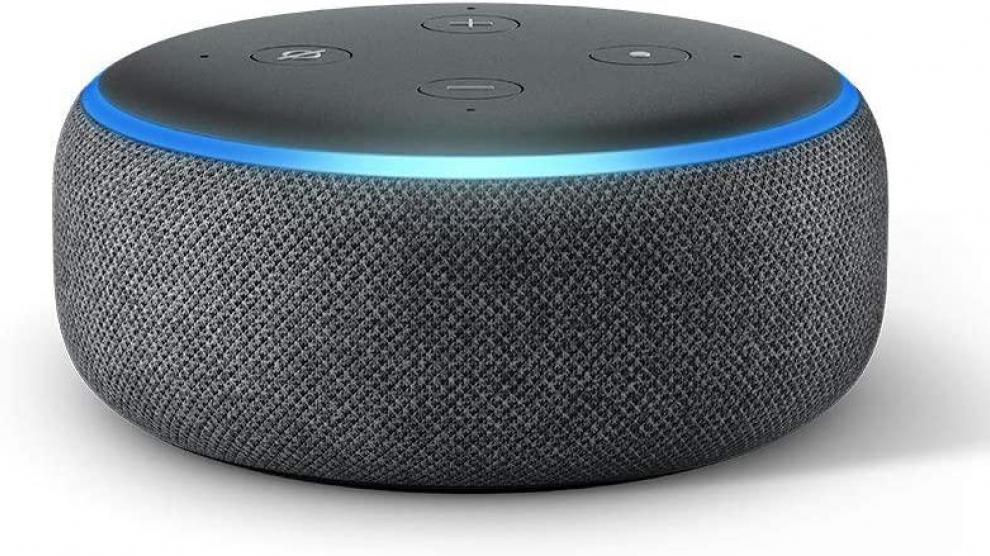
\includegraphics[width=52mm]{figs/Alexa.jpeg}}
      \hspace{2mm}
      \subfigure[Pepper]{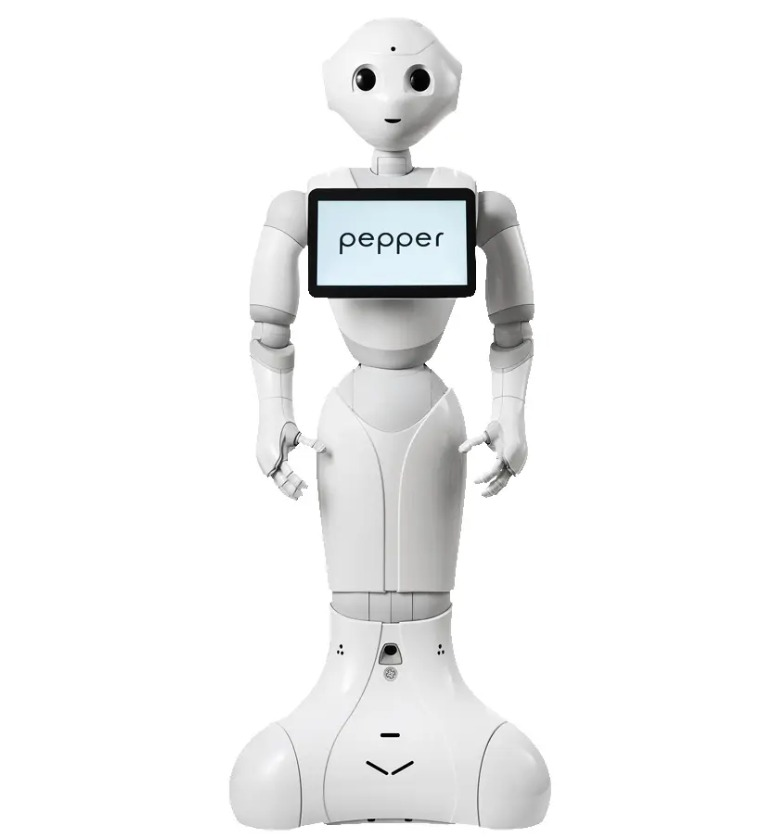
\includegraphics[width=52mm]{figs/Pepper.jpeg}}
      \hspace{2mm}
      \subfigure[Sophia]{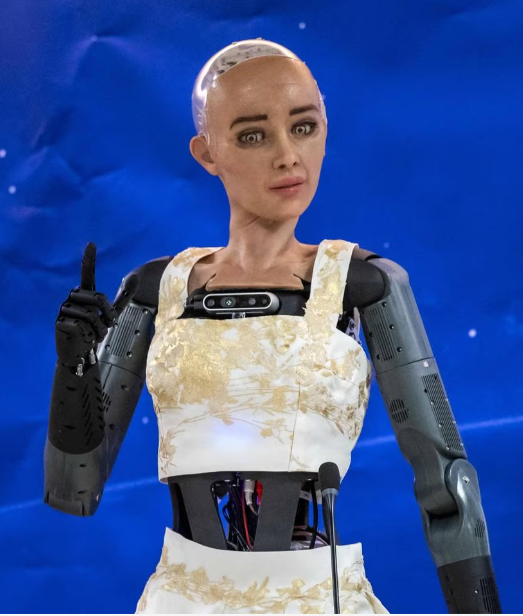
\includegraphics[width=42mm]{figs/Sophia.png}}
    \end{center}
    \caption{Robots de servicio}
    \label{fig:Robots_servicio}
  \end{figure}

Tratando de establecer una división de los robots de servicio, la norma ISO 8373:2012, así como la Ferderación Internacional de Robótica o IFR, propuso clasificarles en diferentes categorías según su función y aplicación en robots para uso doméstico y personal y robots de servicio destinados a un uso profesional \cite{Gonzalez21}, siendo las aplicaciones más importantes las siguientes:

\begin{itemize}
 \item \textit{Limpieza:} Estos robots son máquinas diseñadas específicamente para realizar tareas de limpieza en una variedad de entornos, desde hogares y oficinas hasta centros comerciales, hospitales y más. Suelen estar equipados con sensores y tecnología de navegación que les permite moverse de manera autónoma por el espacio, detectar obstáculos y llevar a cabo actividades de limpieza de manera eficiente. 
 
 \begin{figure} [h!]
  \begin{center}
    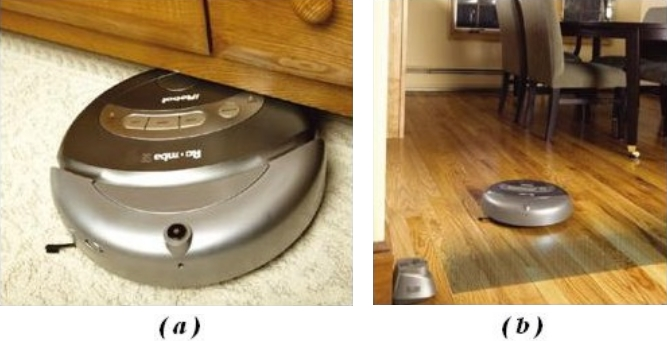
\includegraphics[width=8cm]{figs/roomba}
  \end{center}
  \caption{Robot aspirador Roomba de iRobot.}
  \label{fig:roomba}
\end{figure}\
 
 \item \textit{Inspección y mantenimiento:} Los robots de servicio utilizados en inspección y mantenimiento son máquinas diseñadas para llevar a cabo tareas de supervisión, evaluación y mantenimiento en entornos de infraestructura o áreas de difícil acceso. Estos robots suele ser máquinas autónomas o teleoperadas equipadas con sensores, cámaras y herramientas especializadas que les permiten evaluar, reparar y mantener equipos, estructuras y sistemas en entornos desafiantes o peligrosos. 
 
 \begin{figure}[h!]
    \begin{center}
      \subcapcentertrue
      \subfigure[Spot de Boston Dynamics]{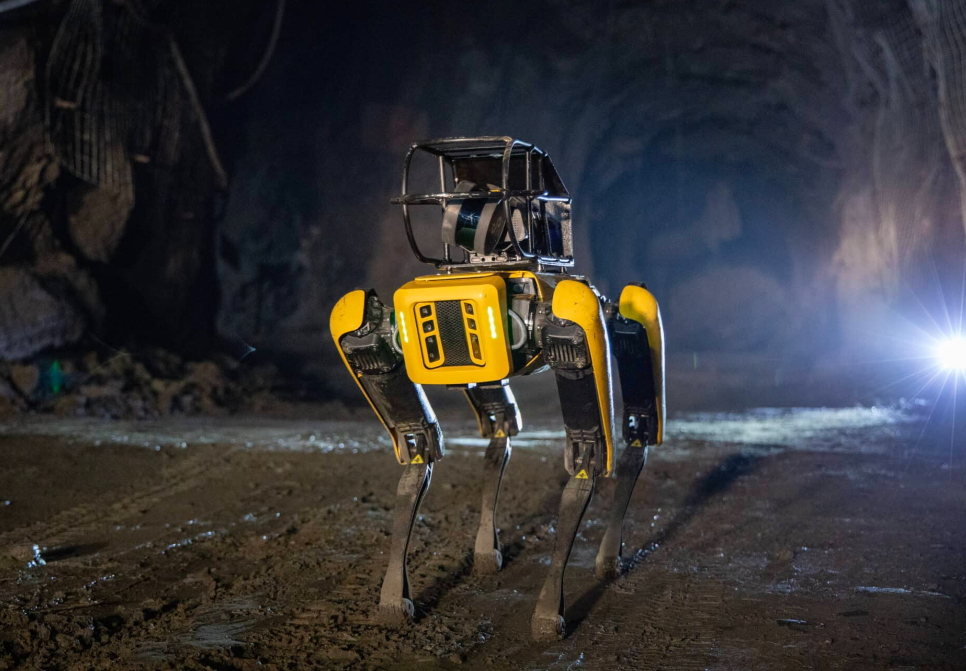
\includegraphics[width=70mm]{figs/Spot.png}}
      \hspace{2mm}
      \subfigure[ROBTET, robot para el mantenimiento de líneas de alta tensión]{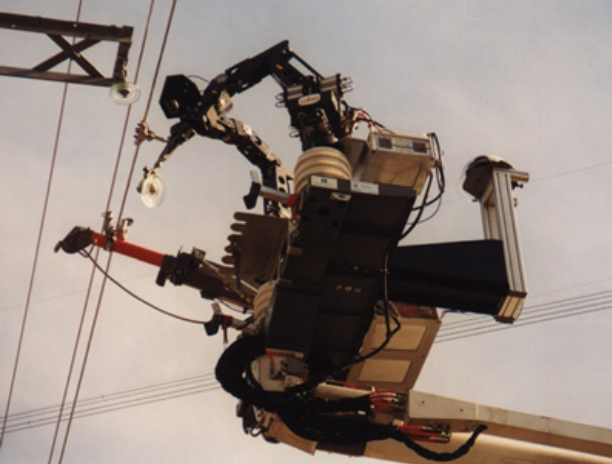
\includegraphics[width=65mm]{figs/ROBTET.png}}
    \end{center}
    \caption{Robots de inspección y mantenimiento.}
    \label{fig:Robots de inspección y mantenimiento}
  \end{figure}
 
 \item \textit{Educación:} Aquellos robots utilizados en educación son robots diseñados para facilitar el aprendizaje y la enseñanza en los diferentes niveles educativos. Estos robots pueden ser utilizados en aulas, bibliotecas y entornos de aprendizaje para ayudar a los estudiantes a adquirir habilidades, fomentar la creatividad y brindar experiencias educativas interactivas.
 
 \pagebreak
 
 \begin{figure}[h!]
    \begin{center}
      \subcapcentertrue
      \subfigure[Robot NAO]{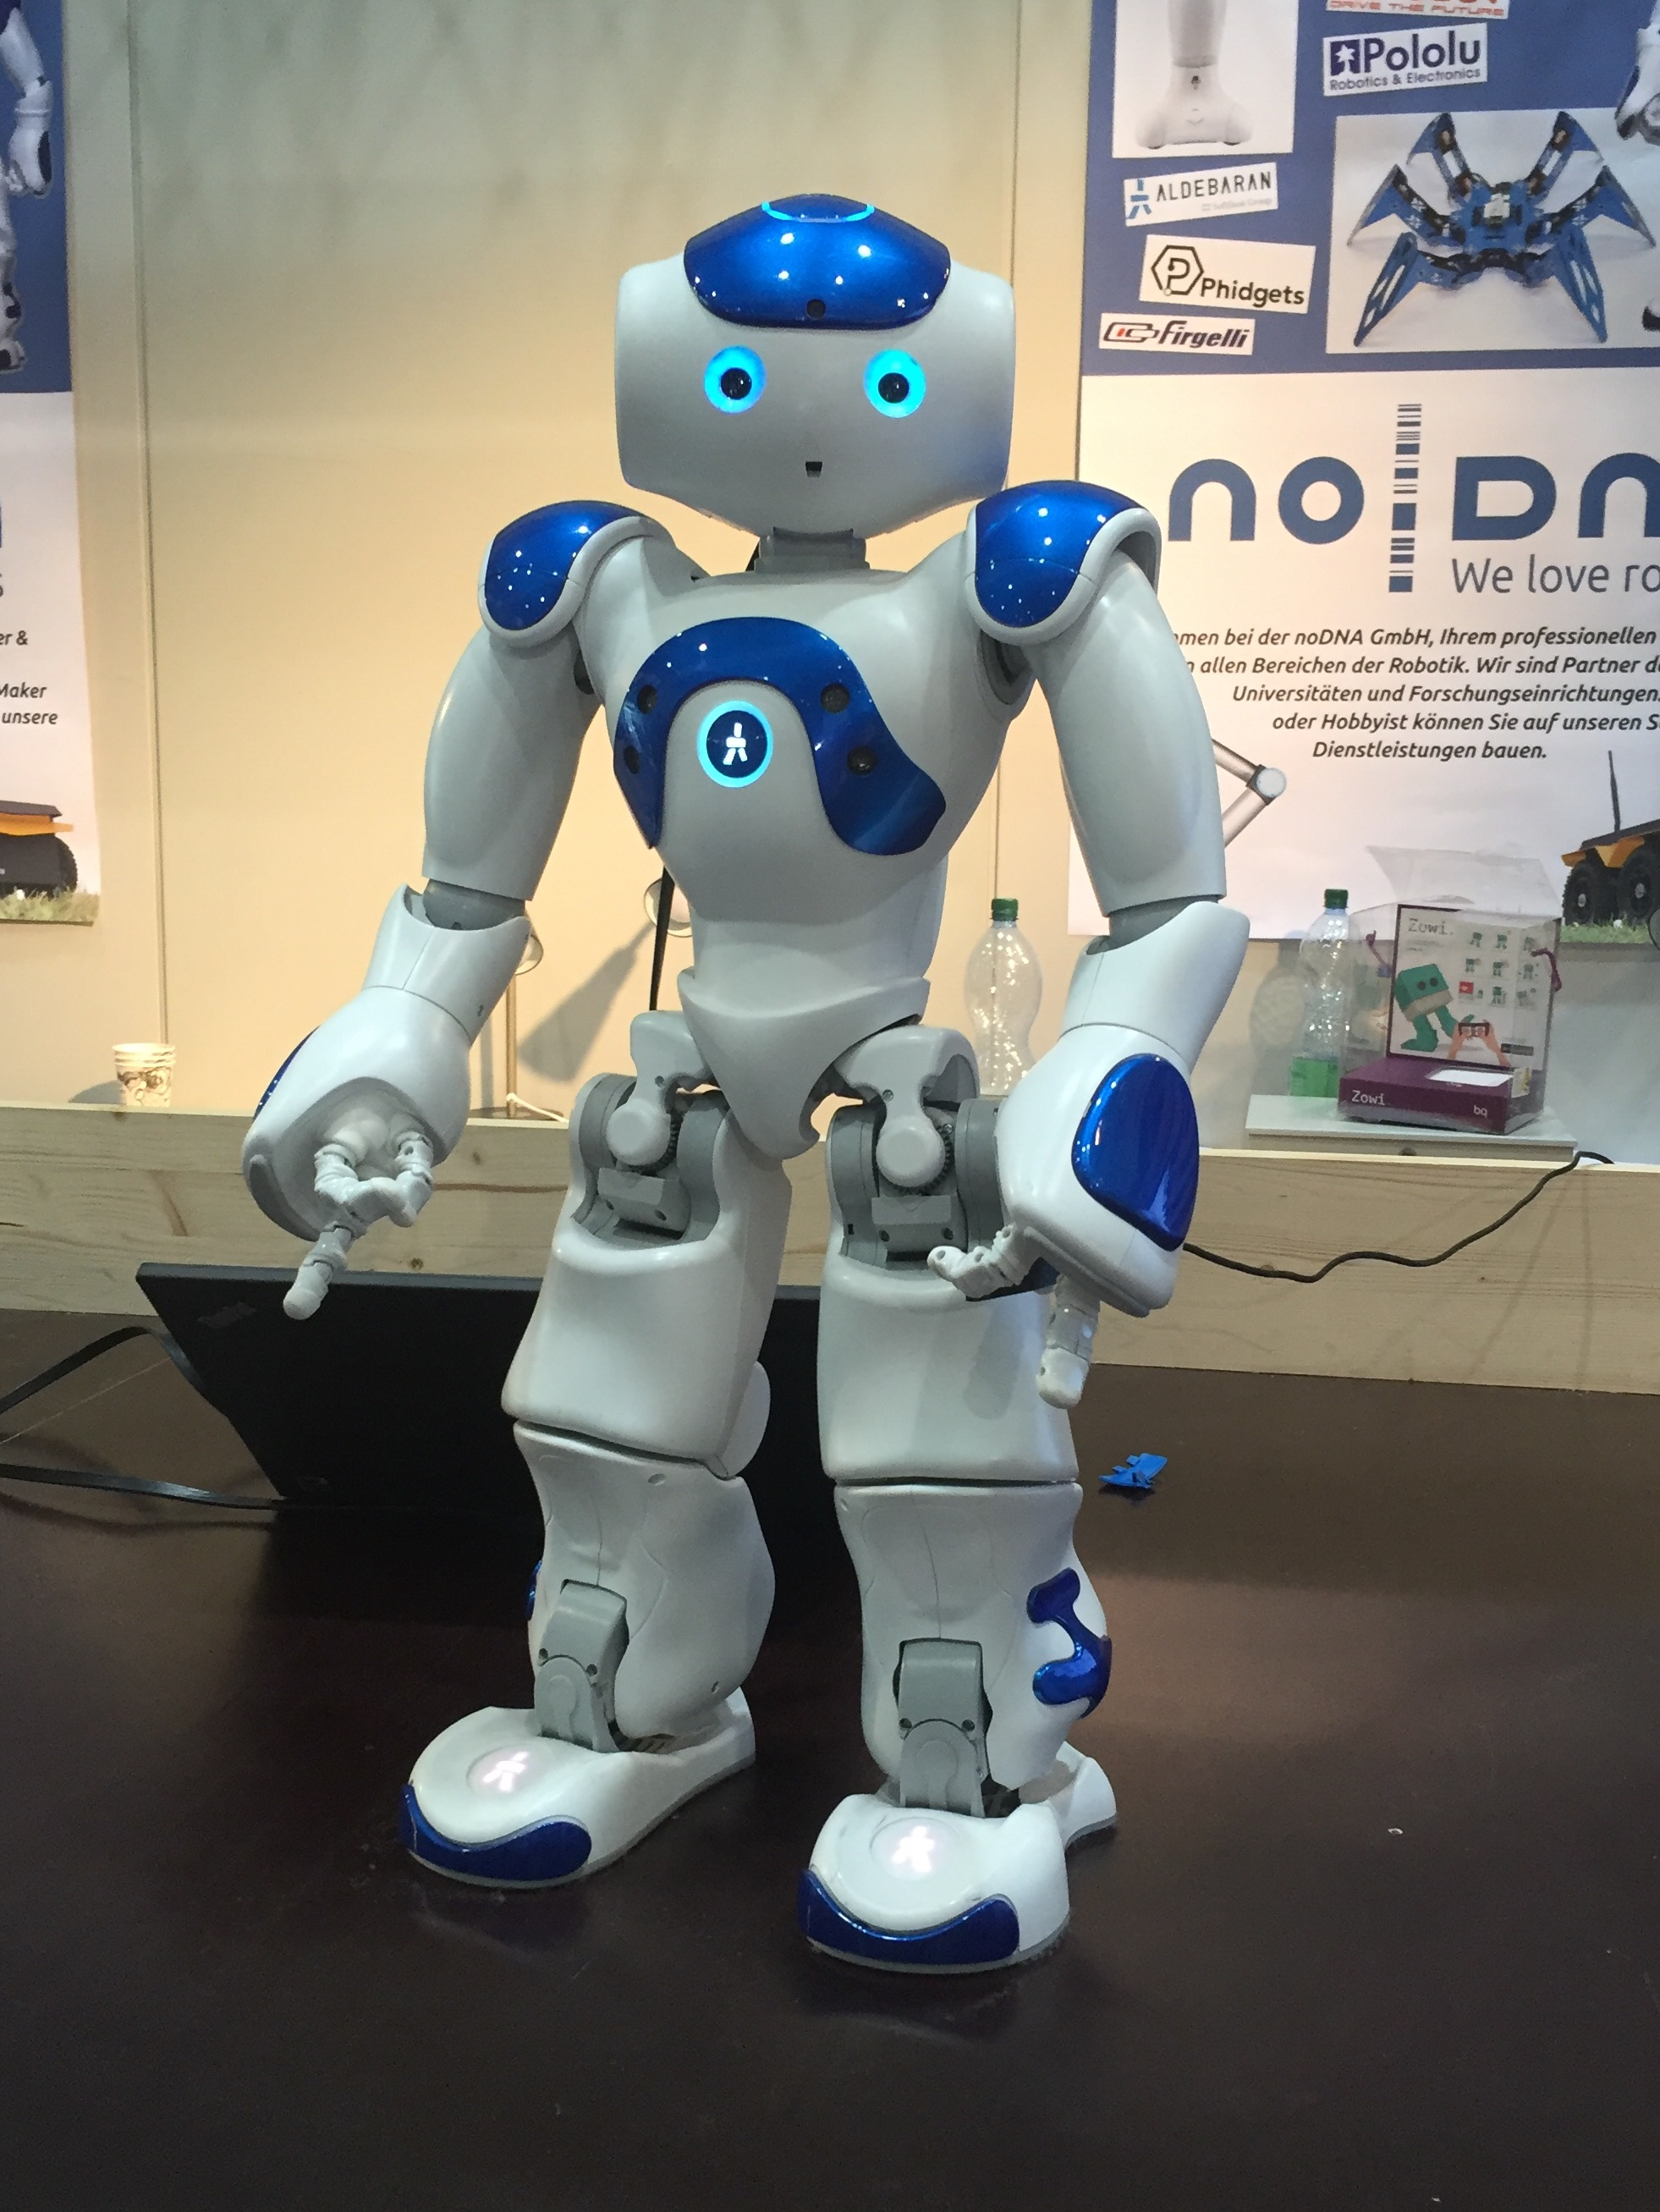
\includegraphics[width=53mm]{figs/Robot NAO.jpg}}
      \hspace{2mm}
      \subfigure[Turtlebot 4]{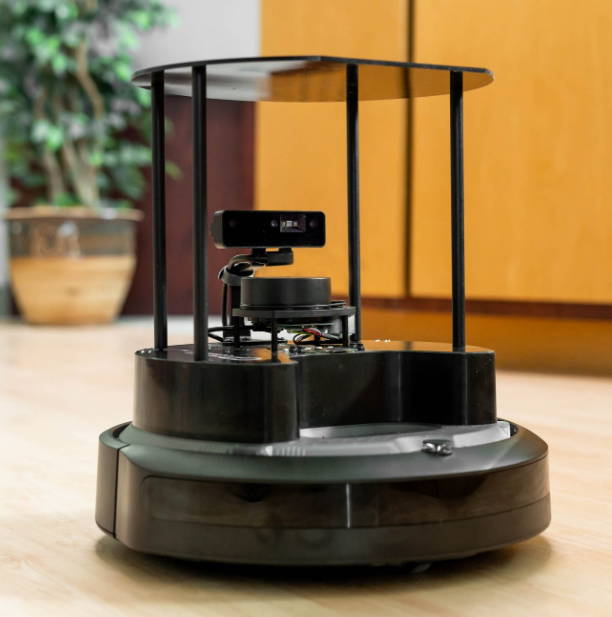
\includegraphics[width=70mm]{figs/Turtlebot 4.png}}
    \end{center}
    \caption{Robots de educación.}
    \label{fig:Robots de educación}
  \end{figure}
 
 \item \textit{Logística:} Los robots de servicio utilizados en logística son robots diseñados para llevar a cabo tareas relacionadas con la gestión y el movimiento de mercancías y productos en entornos de almacenamiento, distribución y transporte. Estos robots desempeñan un papel fundamental en la optimización de la cadena de suministro, mejorando la eficiencia y la precisión en la manipulación de productos. Dentro de los robots de logística empleados para el movimiento de mercancías, se pueden distinguir dos grandes grupos: Vehículos Guiados Automáticos (AGV) y los Robots Móviles Autónomos (AMR).
 
 \item \textit{Entrenenimiento:}
\end{itemize}

\begin{figure} [h!]
    \begin{center}
      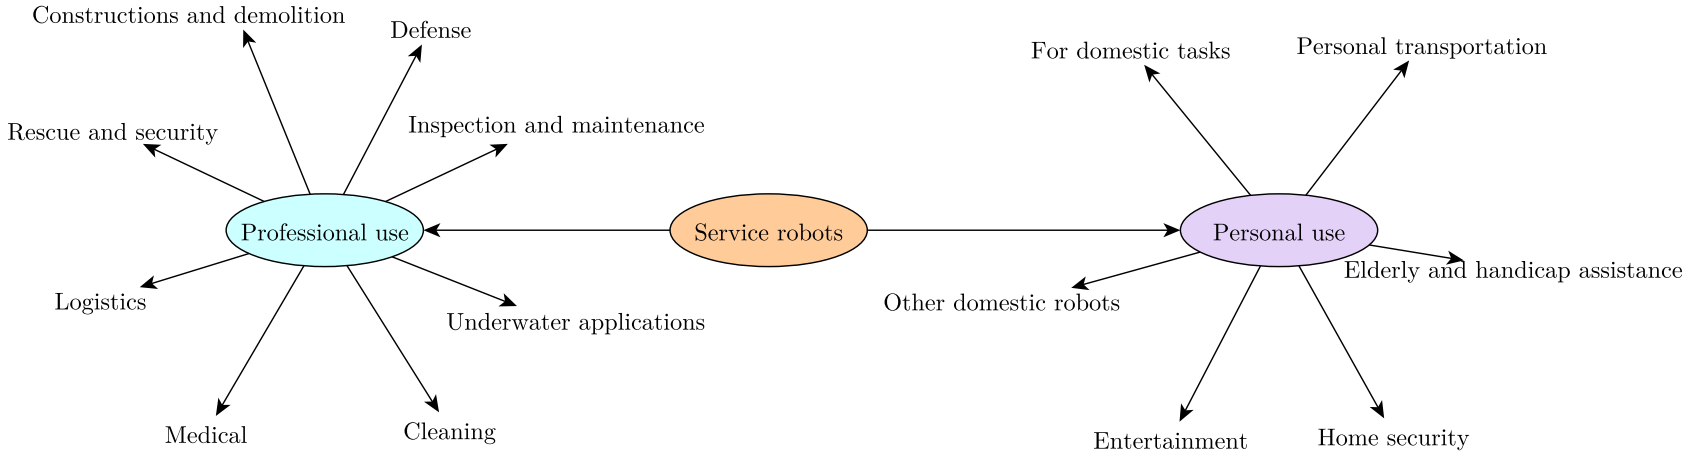
\includegraphics[width=17cm]{figs/Clasificacion robots de servicio.png}
    \end{center}
    \caption{Clasificación de los Robots Servicio según la norma ISO 8373:2012.}
    \label{fig:clasificacion robots servicio}
\end{figure}
   

  
  
\subsection{Robot Médico}
\label{sec:robotica_industrial} 

Se define \textit{robot médico} a aquellos dispositivos electromecánicos que desempeñan parcial o totalmente algunas funciones de los seres humanos o de sus órganos al resolver problemas médicos, ayudando a mejorar la asistencia al paciente y los resultados, a la vez que aumenta la eficiencia operativa \cite{Kraevsky10}.\\

En los textos puedes poner palabras en \textit{cursiva}, para aquellas expresiones en sentido \textit{figurado}, palabras como \textit{robota}, que está fuera del diccionario castellano, o bien para resaltar palabras de una colección: \textit{(a)} es la primera letra del abecedario, \textit{(b)} es la segunda, etc.\\

Al poner las dos líneas del anterior párrafo, este aparecerá separado del anterior. Si no las pongo, los párrafos aparecerán pegados. Sigue el criterio que consideres más oportuno.

\section{Segunda sección}
\label{sec:segundaseccion}

No olvides incluir imágenes y referenciarlas, como la Figura \ref{fig:roomba}.

Ni tampoco olvides de poner las URLs como notas al pie. Por ejemplo, si hablo de la Robocup\footnote{\url{http://www.robocup.org}}.

\subsection{Números}
\label{sec:subseccion}

En lugar de tener secciones interminables, como la Sección \ref{sec:miseccion}, divídelas en subsecciones.

Para hablar de números, mételos en el entorno \textit{math} de \LaTeX, por ejemplo, $1.5Kg$. También puedes usar el símbolo del Euro como aquí: 1.500\euro.

\subsection{Listas}

Cuando describas una colección, usa \texttt{itemize} para ítems o \texttt{enumerate} para enumerados. Por ejemplo:

\begin{itemize}
 \item \textit{Entorno de simulación.} Hemos usado dos entornos de simulación: uno en 3D y otro en 2D.
 \item \textit{Entornos reales.} Dentro del campus, hemos realizado experimentos en Biblioteca y en el edificio de Gestión.
\end{itemize}\

\begin{enumerate}
 \item Primer elemento de la colección.
 \item Segundo elemento de la colección.
\end{enumerate}\

\paragraph{Referencias bibliográficas}
\label{sec:referencias}

% Cita, sobre todo en este capítulo, referencias bibliográficas que respalden tu argumento. Para citarlas basta con poner la instrucción \verb|\cite| con el identificador de la cita. Por ejemplo: libros como \cite{vega12e}, artículos como \cite{vega19b}, URLs como \cite{vega19a}, tesis como \cite{vega18b}, congresos como \cite{vega18a}, u otros trabajos fin de grado como \cite{vega08b}.

Las referencias, con todo su contenido, están recogidas en el fichero \texttt{bibliografia.bib}. El contenido de estas referencias está en formato \texttt{BibTex}. Este formato se puede obtener en muchas ocasiones directamente, desde plataformas como \texttt{Google Scholar} u otros repositorios de recursos científicos.

Existen numerosos estilos para reflejar una referencia bibliográfica. El estilo establecido por defecto en este documento es APA, que es uno de los estilos más comunes, pero lo puedes modificar en el archivo \texttt{memoria.tex}; concretamente, cambiando el campo \verb|apalike| a otro en la instrucción \verb|\bibliographystyle{apalike}|. 

\

\

\

Y, para terminar este capítulo, resume brevemente qué vas a contar en los siguientes.
